\documentclass[12pt]{article}

\usepackage{preamble}
\usepackage{hyperref}
\usepackage{algorithmicx}
\usepackage{algorithm}
\usepackage{algpseudocode}

\begin{document}

\textbf{Final Project.}

Daniel Yao

EN.580.475

\today

\textbf{Introduction.}

Brawl Stars is a 3v3 mobile game developed by Supercell. The competitive format proceeds in two stages: the draft and the gameplay.

First, the game mode (there are six total) is revealed. Two teams, Blue and Red, each independently choose 3 of 97 brawlers to ban. These bans are then revealed. Blue chooses one brawler, Red chooses two brawlers, Blue chooses two brawlers, and then Red chooses one brawler. These brawlers are chosen without replacement so that each team has three brawlers and that these brawlers are unique. The players then play the game mode with their chosen brawlers, and the victor is decided in a best of three contest.

In the past few years, the competitive community has come to jokingly refer to the game as "Draft Stars", due to the increasing importance of the draft stage over the gameplay stage with the addition of new characters.

I address this draft stage. First, I train three models (logistic regression, random forest, and neural network) to predict the game outcome given a draft. I evaluate these three models and select the best one. I then propose a mini-max algorithm to determine the optimal draft strategy using this model. Finally, I address the (many) limitations of my method and draw some conclusions about the state of the game.

\textbf{Methods.}

\textit{Data collection.} I obtained the data during the summer of 2024 through BrawlStarsAPI, though the analysis here is new. There are 5514 games with 82 unique brawlers. (There were fewer brawlers in the game at the time.) All games include at least one top 200 global player.

Since the modes and brawlers are categorical and their is no meaningful order to these categories, the data are one-hot encoded. There are 6 modes and 82 choices for six players, for a total of 
$$6 + 6(82) = 498$$
dimensions. The brawlers are sorted within each team to respect order invariance within teams. The data are permuted so that either team wins with roughly equal probability.

\textit{Logistic regression.} A logistic regression classifier is trained with L2 regularization. The operating point is selected to minimize the distance to the top-left corner of the ROC curve.

\textit{Random forest.} A random forest classifier is trained with 20 trees and Gini impurity criterion. The number of trees is determined empirically. It is found that a small model of 20 trees performs the best. The operating point is selected to minimize the distance to the top-left corner of the ROC curve.

\textit{Neural network.} A neural network is trained with two hidden layers of 32 neurons, ReLU activations, sigmoid output, and BCE loss. The number and size of the hidden layers is determined empirically. It is found that a small model of two hidden layers of 32 neurons performs the best. The operating point is selected to minimize the distance to the top-left corner of the ROC curve.

\textbf{Results.}

The training/testing confusion matrices for each of the three models are shown in the Appendix. The training/testing accuracies, precisions, and recalls are exhibited in the table below. Precision and recall remain fairly balanced in both the training and testing sets for all three models. However, these results show that the models grossly overfit to the training data and fail to maintain 90\% accuracies in testing.

\begin{center}
\begin{tabular}{c|ccc|ccc}
    & \multicolumn{3}{c|}{\textbf{Training}} & \multicolumn{3}{c}{\textbf{Testing}} \\ 
    & Accuracy & Precision & Recall & Accuracy & Precision & Recall \\ 
    \hline
    % Your data rows go here
    Logistic regression & 0.65 & 0.65 & 0.66 & 0.53 & 0.51 & 0.57 \\
    Random forest & 0.92 & 0.92 & 0.92 & 0.61 & 0.58 & 0.65 \\
    Neural Network & 0.92 & 0.97 & 0.86 & 0.61 & 0.59 & 0.61 \\
\end{tabular}
\end{center}

The testing accuracies of each of the three models are shown below with 95\% confidence intervals. A baseline positive rate reference is shown, which depicts the accuracy of always predicting the (training set) majority class. The random forest and neural network perform significantly better than the baseline positive rate at a significance level of $\alpha = 0.05$.

\begin{center} 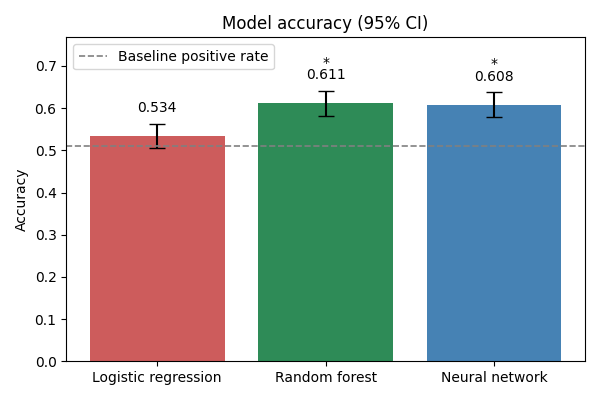
\includegraphics[width=4in]{"../output/acc.png"} \end{center}

The $R^{2}$s of each of the models for the testing set is shown below. The $R^{2}$ is computed as 
$$R^{2} = 1 - \frac{y^{T}\hat{y}}{y^{T}y},$$
where $y$ is the vector of true labels and $\hat{y}$ is the vector of predicted probabilities. This value roughly corresponds to the proportion of variance explained by the model. The random forest has the best $R^{2}$, explaining $6.6\%$ of the total variance.

\begin{center} 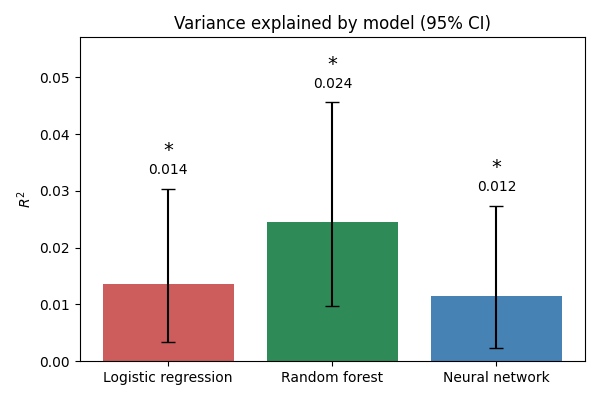
\includegraphics[width=4in]{"../output/r2.png"} \end{center}

\textbf{Discussion.}

The logistic regression is no better than always guessing the majority class. The random forest and neural network perform similarly, with accuracies of $61.1\%$ and $60.8\%$ and $R^{2}$s of $0.066$ and $0.057$, respectively. Neither model achieves very high accuracy, but this is expected because the draft is not the only factor that determines the outcome of a game.

Strong conclusions are hard to draw from these data. Though the outcome of a match can be predicted better than chance from only the draft, there is the possibility that players who are better mechanically are also better draft-wise. Nevertheless, a rough heuristic yields that these data are compatible with the explanation that (at least) 20\% of games are determined entirely by the draft while the other (at most) 80\% of games are determined entirely by mechanics. This matches my experience from playing the game.

Another limiation is that the data only included 5,414 games, while there are 
$$\binom{82}{3,3,76} \big/ 2 = 3,501,618,120$$
total match ups (A vs B is identical to B vs A). As such, almost all possible match ups are not represented in the data set. The models therefore operates almost entirely out of distribution. Nevertheless, the random forest and neural network are able to somewhat generalize to unseen data with $61.1\%$ and $60.8\%$ accuracy, respectively.

\textbf{Application.} 

Now that a model for predicting the outcome of a match given a draft is provided, this model can be used to advise a team how to draft to maximize its victory probability. The minimax algorithm is a deterministic algorithm that finds the optimal strategy to maximize a utility function in a two-player game. The algorithm features two agents, a maximizer and a minimizer, who choose the strategy that maximizes/minimizes the guaranteed utility regardless of the opponent's strategy. The minimax with alpha-beta pruning algorithm is a depth-first search of the action space, which prunes branches that are worse than the previously found maximum/minimum.

In this case, the actions are to select brawlers in accordance to the draft rules, and the utility function is the victory probability predicted by a model. The random forest model is found to work the best for this application. The ban phase is ignored to reduce the state space. The minimax algorithm is described in the Appendix.

Nevertheless, the state space remains very large, containing 
$$\binom{82}{3,3,76} = 7,003,236,240$$
possible match ups (A vs B is not identical to B vs A). A full-depth search is computational infeasible, but this issue can be resolved by precomputing lookup tables or by parallelization. The focus of this project is not on the minimax algorithm, so the algorithm is only implemented to function, starting from pick $4$. An example draft is shown, where $(*)$ marks picks that are chosen by the minimax algorithm.

\begin{center}
\begin{tabular}{c|ccc|ccc}
    & \multicolumn{3}{c|}{\textbf{Team 1}} & \multicolumn{3}{c}{\textbf{Team 2}} \\ 
    Mode & Pick 1 & Pick $4^{*}$ & Pick $5^{*}$ & Pick 2 & Pick 3 & Pick $6^{*}$ \\
    Bounty & Brock & 8-Bit & Belle & Gene & Max & Bonnie \\
    \hline
    \textbf{Utility} & & 55\% & &  & 45\% & 
\end{tabular}
\end{center}

\textbf{Conclusion.}

Nevertheless, it is impressive that 

\textbf{Code availability.}

\href{https://github.com/dyao13/580_475_FA25}{github.com/dyao13/580\_475\_FA25}

\newpage \textbf{References.}

Brawl Stars. (2017). Supercell.

\newpage \textbf{Appendix.}

\begin{center} 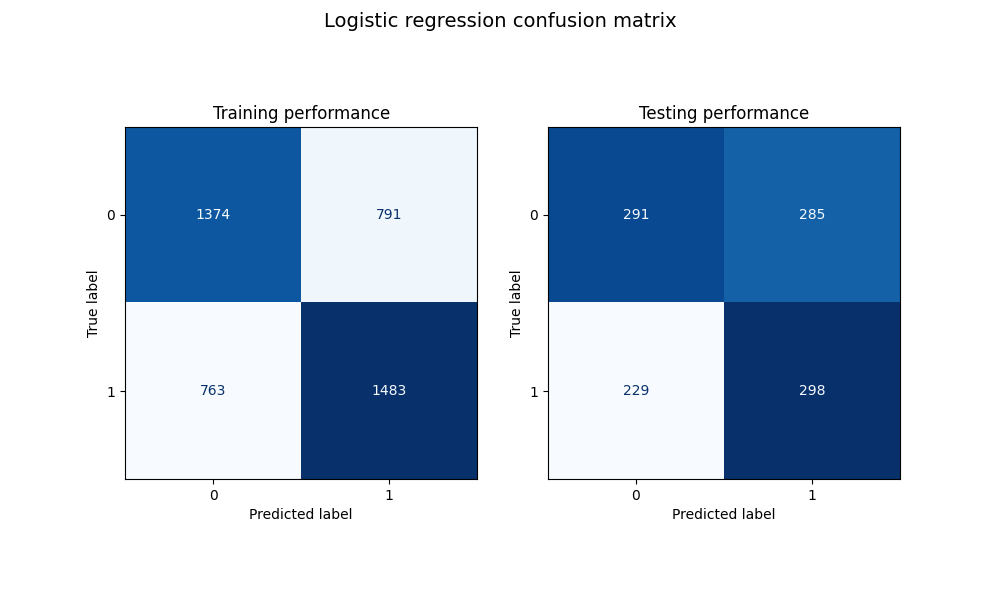
\includegraphics[width=6in]{"../output/lr_training_testing_confusion_matrices.png"} \end{center}

\begin{center} 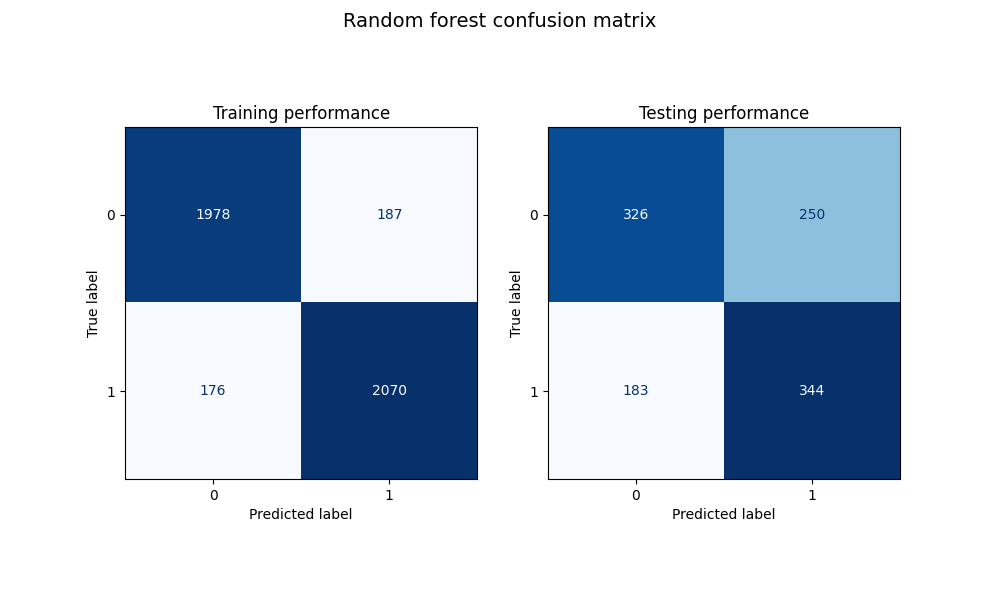
\includegraphics[width=6in]{"../output/rf_training_testing_confusion_matrices.png"} \end{center}

\begin{center} 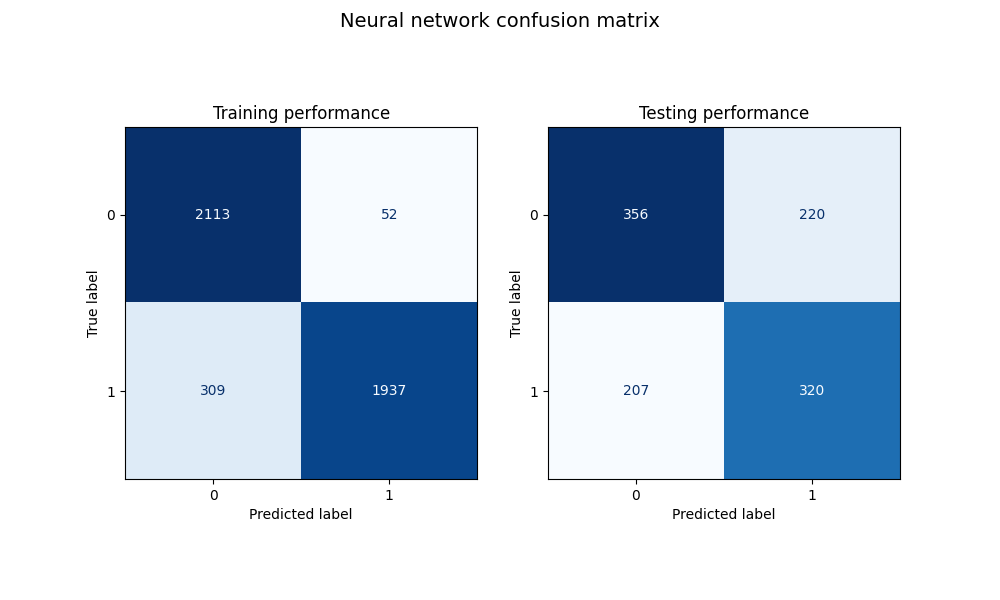
\includegraphics[width=6in]{"../output/nn_training_testing_confusion_matrices.png"} \end{center}

\begin{algorithm}[H]
\caption{Minimax with $\alpha$–$\beta$ pruning}
\label{alg:alphabeta}
\begin{algorithmic}[1]
\Function{Minimax}{$s, d, \alpha, \beta, \text{isMaximizer}$}
    \If{$\textsc{Terminal}(s)$ \textbf{ or } $d = 0$}
        \State \Return $\textsc{Utility}(s)$
    \EndIf
    \If{\text{isMaximizer}}
        \State $v \gets -\infty$
        \ForAll{$a \in \textsc{Actions}(s)$}
            \State $v \gets \max\big(v,\ \textsc{Minimax}(\textsc{Result}(s,a),\ d-1,\ \alpha,\ \beta,\ \textbf{false})\big)$
            \State $\alpha \gets \max(\alpha, v)$
            \If{$\alpha \ge \beta$} \State \textbf{break}
            \EndIf
        \EndFor
        \State \Return $v$
    \Else
        \State $v \gets +\infty$
        \ForAll{$a \in \textsc{Actions}(s)$}
            \State $v \gets \min\big(v,\ \textsc{Minimax}(\textsc{Result}(s,a),\ d-1,\ \alpha,\ \beta,\ \textbf{true})\big)$
            \State $\beta \gets \min(\beta, v)$
            \If{$\alpha \ge \beta$} \State \textbf{break}
            \EndIf
        \EndFor
        \State \Return $v$
    \EndIf
\EndFunction
\end{algorithmic}
\end{algorithm}

\end{document}